% ==============================================================================
% FICHIER : chapitre7.tex
% Description : Chapitre 7 (Sprint 4) : Espace Gamification, Clôture et Historique Citoyen
% Auteurs : Dhia Fersi & Mohamed Iyed Amiri (ISET Bizerte)
% Organisme d'accueil : HRMAPS
% ==============================================================================

\chapter[Sprint 4 : Gamification et Historique]{Sprint 4 : Espace Gamification, Clôture et Historique}

\section*{Introduction}
\addcontentsline{toc}{section}{Introduction}
La réussite d'une plateforme participative comme \textit{SafeCity-Connect} repose sur l'interaction active et transparente entre les citoyens, la municipalité et les services techniques. L'objectif du Sprint 4 est de finaliser le cycle de vie de l'incident. Ce cycle comprend le téléversement de la photo preuve par le département technique, la modération de cette preuve par l'administrateur (acceptation ou rejet motivé avec saisie obligatoire d'une raison), et la possibilité pour le citoyen de commenter et d'évaluer la qualité de la réparation (\textit{review fixes}). De plus, ce sprint implémente le suivi global par une frise chronologique détaillée (\textbf{Timeline}) pour chaque anomalie, réservée à la consultation de l'administrateur. Ce chapitre présente le backlog, la modélisation fonctionnelle, les diagrammes UML, et l'implémentation de la logique de clôture, de modération et de commentaires.

% ------------------------------------------------------------------------------
% 1. BACKLOG SPRINT 4
% ------------------------------------------------------------------------------
\section{BACKLOG Sprint 4}
Le Backlog du Sprint 4 consolide les récits utilisateurs liés aux chantiers, à la modération finale et aux retours citoyens :
\begin{itemize}
    \item \textbf{US09 -- Photo preuve de fixation (Département)} : Permettre à l'agent technique d'uploader une photo de l'anomalie réparée pour clore son intervention.
    \item \textbf{US10 -- Modération et Raison de Rejet (Admin)} : Permettre à l'administrateur de valider ou de refuser la réparation soumise par le département en saisissant une raison obligatoire enregistrée dans la timeline de l'incident.
    \item \textbf{US11 -- Commentaires et Notation de la réparation (Citoyen)} : Permettre aux citoyens d'écrire des commentaires sur l'incident et de donner leur avis après la résolution de l'anomalie (\textit{review fixes}).
\end{itemize}

% ------------------------------------------------------------------------------
% 2. ANALYSE ET SPÉCIFICATION DES BESOINS
% ------------------------------------------------------------------------------
\section{Analyse et spécification des besoins}

\subsection{Diagramme de cas d'utilisation}
La figure \ref{fig:uc_sprint4} présente les cas d'utilisation liés à l'authentification des agents, la modération des preuves de fixation, la rédaction de commentaires et l'attribution finale des points de gamification.

\begin{figure}[H]
    \centering
    \framebox[\textwidth]{\vbox to 5.5cm{\vfill\hbox to \textwidth{\hss\textbf{[Figure : Diagramme de Cas d'Utilisation -- Sprint 4 (Clôture et Avis Citoyens)]}\hss}\vfill}}
    \caption{Diagramme de cas d'utilisation : Sprint 4}
    \label{fig:uc_sprint4}
\end{figure}

\subsection{Description textuelle}
Voici la description textuelle du cas d'utilisation principal \textbf{« Modérer la résolution d'un incident »} :
\begin{itemize}
    \item \textbf{Acteur} : Administrateur.
    \item \textbf{Préconditions} : L'incident est à l'état « A\_VALIDER\_FIX » (le département technique a téléversé sa photo preuve).
    \item \textbf{Scénario nominal} :
    \begin{enumerate}
        \item L'administrateur ouvre l'interface de modération de la réparation sur la console web.
        \item Il compare la photo initiale (avant) et la photo preuve (après) fournie par les agents.
        \item \textbf{Cas A (Acceptation)} : L'administrateur valide la réparation. Le statut passe à « RESOLVED », la timeline est mise à jour, et le citoyen reçoit automatiquement ses points d'impact.
        \item \textbf{Cas B (Rejet)} : L'administrateur refuse la réparation, saisit obligatoirement un motif (ex : « Bitume mal tassé, fissure encore visible ») et valide. Le statut repasse à « EN\_COURS » pour ré-intervention, et la raison du refus est consignée dans la timeline de l'incident pour le suivi de l'administration.
    \end{enumerate}
    \item \textbf{Scénarios alternatifs} : Si l'administrateur valide l'incident sans saisir de motif en cas de rejet, le système affiche un message d'erreur et bloque la validation.
\end{itemize}

% ------------------------------------------------------------------------------
% 3. PRÉSENTATION ÉCRAN IHM
% ------------------------------------------------------------------------------
\section{Présentation écran IHM}
L'interface de l'application mobile Flutter permet aux citoyens de donner leur avis sur les réparations et d'échanger des commentaires :

\begin{figure}[H]
    \centering
    \framebox[\textwidth]{\vbox to 6.5cm{\vfill\hbox to \textwidth{\hss\textbf{[Capture d'écran : Application Flutter Citoyen -- Section Commentaires et Avis sur la Réparation (sans timeline)]}\hss}\vfill}}
    \caption{Interface de l'historique citoyen avec statut et commentaires}
    \label{fig:ihm_gamification}
\end{figure}

% ------------------------------------------------------------------------------
% 4. DIAGRAMME DE SÉQUENCE
% ------------------------------------------------------------------------------
\section{Diagramme de sequence}
La figure \ref{fig:seq_sprint4} décrit le flux d'informations lors du rejet d'une réparation par l'administrateur avec motif, sa mise à jour en base de données et sa consignation dans la timeline d'incident de l'administrateur.

\begin{figure}[H]
    \centering
    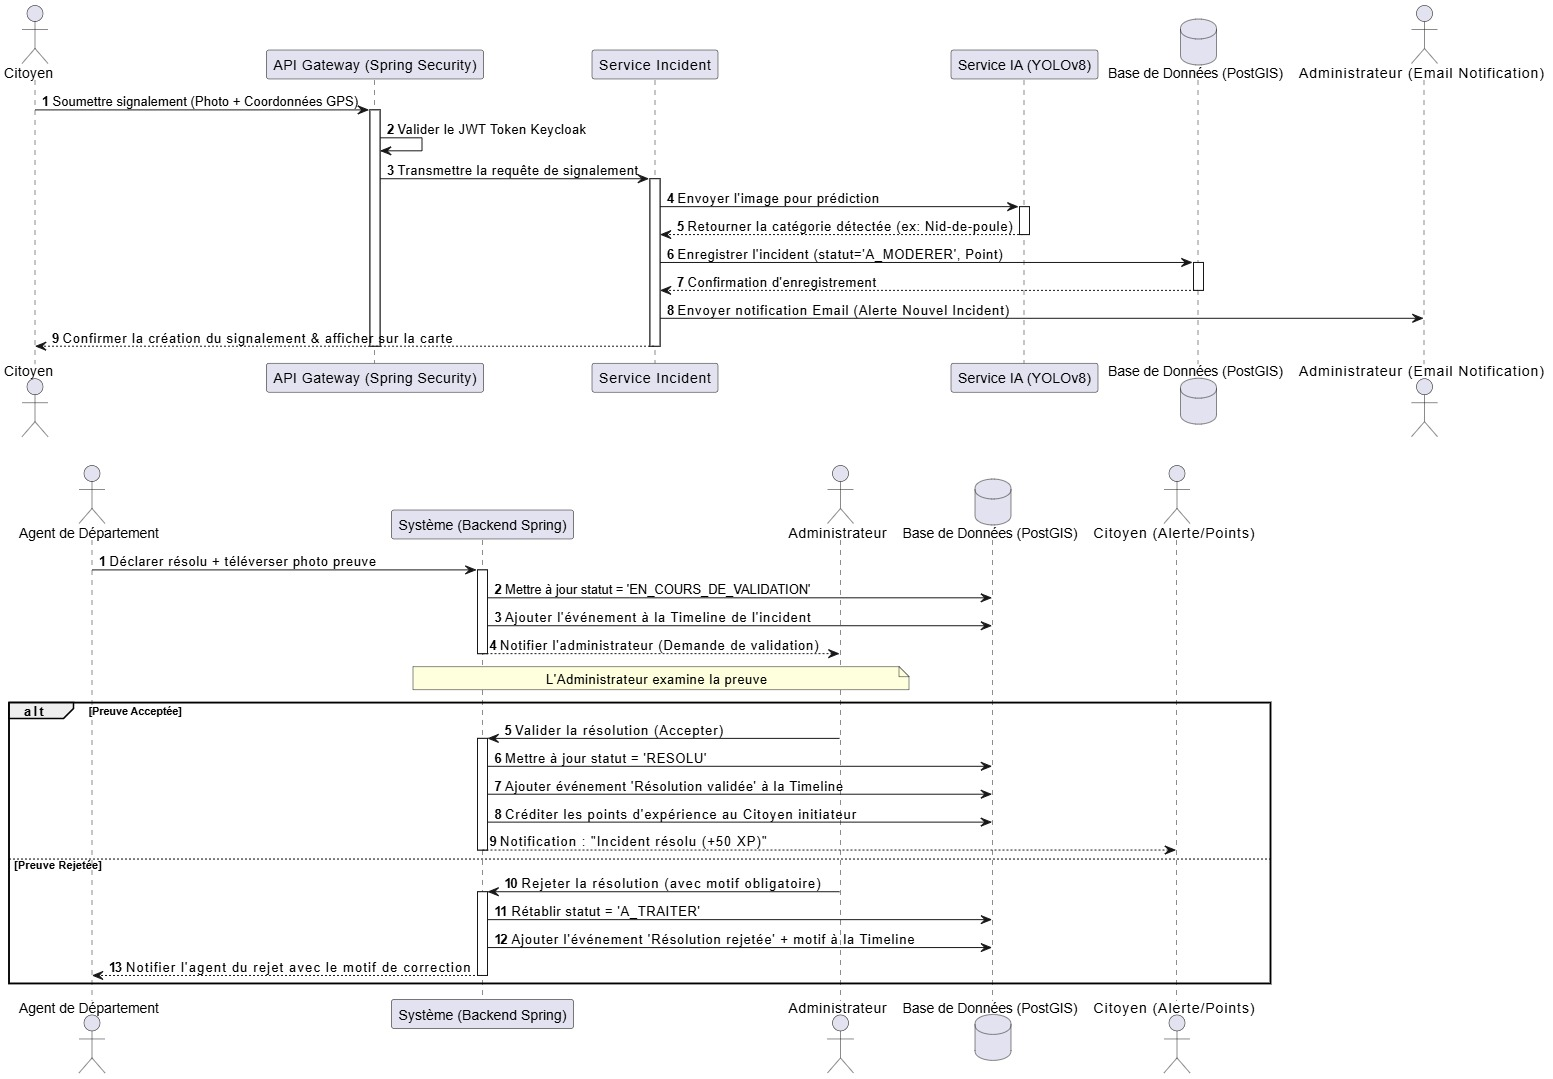
\includegraphics[width=\textwidth]{seq_resolution_moderation.jpg}
    \caption{Diagramme de séquence : Modération et Retours citoyens}
    \label{fig:seq_sprint4}
\end{figure}

% ------------------------------------------------------------------------------
% 5. DIAGRAMME DE CLASSES
% ------------------------------------------------------------------------------
\section{Diagramme de classes}
La figure \ref{fig:class_sprint4} détaille la structure statique du code gérant l'historique des statuts (Timeline), les entités de commentaires (\texttt{Comment}) et les notes d'évaluation (\texttt{FixReview}).

\begin{figure}[H]
    \centering
    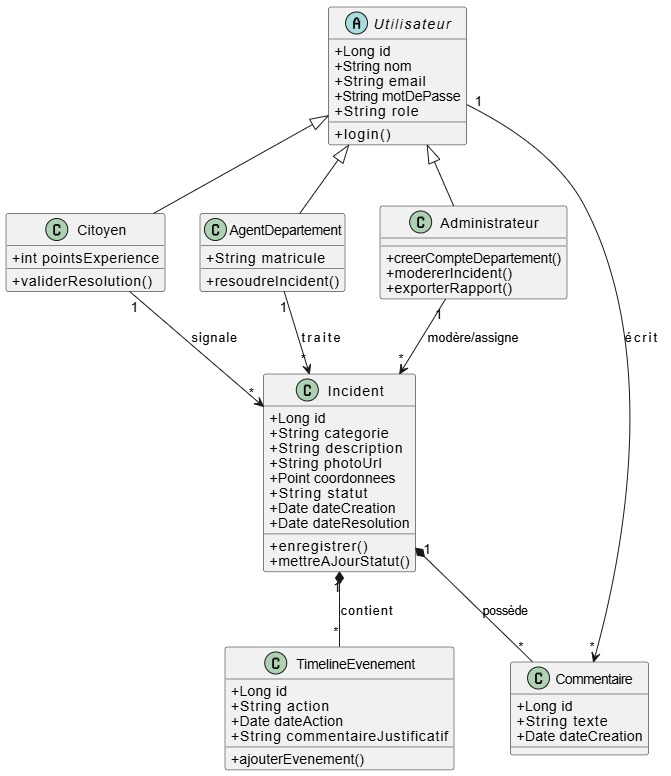
\includegraphics[width=0.9\textwidth]{classes_sprint4.jpg}
    \caption{Diagramme de classes du Sprint 4}
    \label{fig:class_sprint4}
\end{figure}

% ------------------------------------------------------------------------------
% 6. RÉALISATION
% ------------------------------------------------------------------------------
\section{Réalisation}

\subsection{Modélisation de la Timeline en Base de Données}
Chaque incident possède un historique d'états géré par la table \texttt{table_incident_timeline} :
*   \texttt{id} (BIGINT, PK)
*   \texttt{incident_id} (FK vers la table incident)
*   \texttt{status} (VARCHAR, ex : SOUMIS, AFFECTE, A_VALIDER_FIX, RESOLVED)
*   \texttt{comment} (TEXT, stocke le motif du rejet de l'Admin ou les notes d'affectation)
*   \texttt{actor_name} (VARCHAR, nom de l'acteur ayant déclenché l'événement)
*   \texttt{created_at} (TIMESTAMP)

\subsection{Implémentation de la Modération et des Commentaires}
La couche service Spring Boot implémente la modération finale de la preuve de fixation :
\begin{verbatim}
@Service
public class ModerationService {
    @Autowired
    private IncidentRepository incidentRepository;
    @Autowired
    private TimelineRepository timelineRepository;
    @Autowired
    private UserProfileRepository userRepository;

    @Transactional
    public void moderateFixation(Long incidentId, boolean isAccepted, String reason, String adminName) {
        Incident incident = incidentRepository.findById(incidentId)
            .orElseThrow(() -> new ResourceNotFoundException("Incident non trouvé"));

        IncidentTimeline log = new IncidentTimeline();
        log.setIncident(incident);
        log.setActorName(adminName);
        log.setCreatedAt(LocalDateTime.now());

        if (isAccepted) {
            incident.setStatus("RESOLVED");
            log.setStatus("RESOLVED");
            log.setComment("Réparation validée par l'administration.");
            
            // Créditer les points au citoyen
            UserProfile citizen = incident.getUser();
            citizen.setImpactPoints(citizen.getImpactPoints() + incident.getCategory().getBasePoints());
            userRepository.save(citizen);
        } else {
            // Rejeter la fixation et remettre en cours pour nouvelle intervention
            incident.setStatus("EN_COURS");
            log.setStatus("EN_COURS");
            log.setComment("Réparation rejetée. Motif : " + reason); // Motif de rejet obligatoire
        }
        
        incidentRepository.save(incident);
        timelineRepository.save(log);
    }
}
\end{verbatim}

\subsection{Enchaînement des interfaces réalisées}
Sur l'application mobile Flutter, le citoyen ouvre un incident. Il visualise son statut de résolution (fixé ou non) directement sur la carte interactive. Si l'incident est résolu (avec photo preuve validée), le citoyen peut alors taper un commentaire (ex : « Merci pour la réactivité, le trou est bien bouché ! ») ou attribuer une note sous forme d'étoiles pour évaluer la qualité du correctif, favorisant la transparence démocratique locale. L'accès à la timeline chronologique détaillée de l'incident et aux détails de modération reste réservé à la console d'administration.

\section*{Conclusion}
Le Sprint 4 clôture le cycle de vie de la plateforme \textit{SafeCity-Connect} en intégrant un workflow de modération rigoureux des réparations et un espace de commentaires interactif. L'enchaînement des interfaces Flutter et Angular garantit un flux d'information transparent et continu : du signalement citoyen géo-localisé à la fixation par photo preuve, validée par l'administration et commentée par la communauté.
